%!TEX root =  ../main.tex

\subsection{Difference Quotient}


\objective{Explain the various forms of the difference quotient and their meaning.}


To all appearances, limits seem to be about incredibly precise --- more precise
than anything in our universe --- or unmeasurably large inputs of functions.
This would seem to offer us nothing useful about the world we actually find ourselves
in.  Such is not the case, however.

If we want to know about the rate of change of a function, we must typically ask 
``over what interval?''  We might suspect that there is a moment on the graph below
($x\approx.25$) where the average rate of change is 0.  How might we prove that?
We would have to travel some further amount in the $x$ direction, which would
produce some change in the $y$ value, because the rate of change is $\frac{\Delta y}
{\Delta x}$.

\begin{figure}
\begin{center}
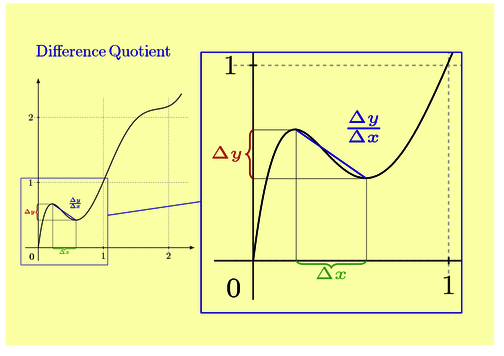
\includegraphics[scale=0.6]{dq.png}
% http://www.texample.net/tikz/examples/difference-quotient/
\caption{The difference quotient, as $\Delta x$ approaches 0\cite{tikzdq}.}
\end{center}
\end{figure}

In single-variable calculus, the difference quotient is usually the name for the expression
\begin{equation}
\lim_{h\rightarrow0}\frac {f(x+h)-f(x)}{(x+h)-x}
\end{equation}

What does this represent?  We are looking for the rate of change of the function.  We begin
by inputting $x$ (and, of course, receiving an output of $f(x)$).  We then move over a tiny 
amount and measure the change in output, over the change in input.  That tiny amount is called
$h$, and we take the limit as $h$ goes to 0.

Because we are evaluating the entire function this way, if we are able to answer the limit, 
we will receive a new function as out answer.  This function is called the \textbf{derivative} of
$f(x)$.


\begin{derivation}{Derivative}
The derivative of a function $f(x)$ may be denoted $f'(x)$.  This style of writing is
called \textbf{Lagrange's notation}, after Joseph-Louis Lagrange
\end{derivation}


\begin{figure}
\begin{center}
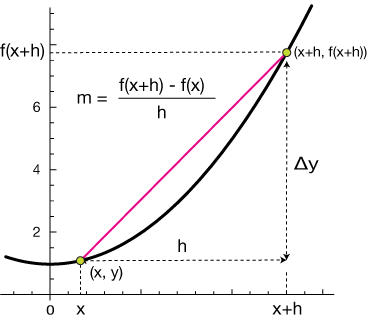
\includegraphics[scale=0.9]{deriv.png}
\caption{The difference quotient produces a secant line \cite{derivativedefinition}.}
\end{center}
\end{figure}

Sometimes it is too difficult or time consuming to find the entire derivative equation.
We might want to find the derivative at one location only, typically called $c$

\begin{equation}
\lim_{x\rightarrow c}\frac{f(x)-f(c)}{x-c}
\end{equation}

These tend to be much easier to solve, as they are typically removable discontinuities
of the kind we solved in §2.1

\subsection{Theorems of Limits}
Let's us generalize the properties of limits we have seen in action this chapter:
\begin{enumerate}
\item The limit of a product is the same as a product of limits
\item The limit of a sum is the same as a sum of limits
\item The limit of a quotient is the same as a quotient of limits (but $\ne 0$)
\item The limit of a constant times a function is the same as a constant times a limit
\item the limit of a constant is a constant
\end{enumerate}
